% !TEX root = ./Basilisk-ThrusterForces-20160627.tex
\section{Module Description}
\begin{figure}[htb]
	\centerline{
	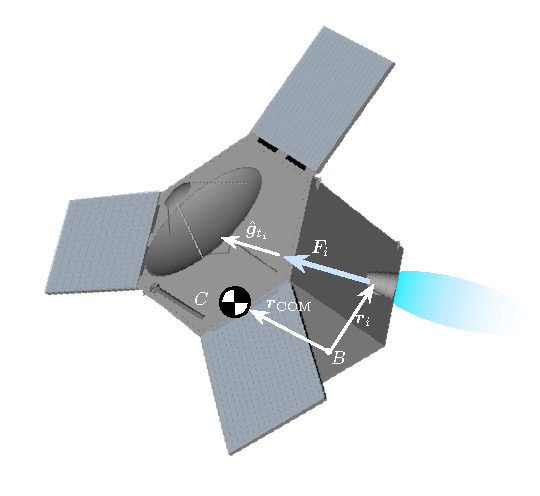
\includegraphics[]{Figures/thrusterNotation}
	}
	\caption{Illustration of the Spacecraft Thruster Notation}
	\label{fig:thruster}
\end{figure}

\subsection{Introduction}
\subsubsection{Torque Control Axes}
This technical note describes a general algorithm that maps a desired ADCS external control torque $\bm L_{r}$ onto force commands for a cluster of thrusters.  Let $\hat{\bm c}_{j}$ be the axis about which the thrusters are to produce the desired torque.  The matrix of $N_{c}$ thruster axes rows is then given by
\begin{equation}
	[C]  = \begin{bmatrix}
		\hat{\bm c}_{1} \\ \vdots \\ \hat{\bm c}_{N_{c}}
	\end{bmatrix}
\end{equation}
The module can accept up to 3 orthogonal control axis $\hat{\bm c}_{j}$.  Let $\bar{\bm L}_{r}$ be the three-dimensional reduced set of $\bm L_{r}$ onto the set of control axes written in the body-frame, given by:
\begin{equation}
	{}^{\mathcal{B}}\bar{\bm L}_{r} = [C]^{T} [C] {}^{\mathcal{B}}\bm L_{r}
\end{equation}
The goal of the thruster mapping strategy is to find a set of $\bm F$ thruster forces that yield $\bar{\bm L}_{r}$.  

\subsubsection{Thruster to Torque Mapping Matrix}
The $i^{\text{th}}$ thruster location relative to the spacecraft point $B$ is given by $\bm r_{i}$ as illustrated in Figure~\ref{fig:thruster}.  The unit direction vector of the thruster force is $\hat{\bm g}_{t_{i}}$, while the thruster force is given by
\begin{equation}
	\label{eq:th:1}
	\bm F_{i} = F_{i} \hat{\bm g}_{t_{i}}
\end{equation}
The toque vector produced by each thruster about the body fixed point $C$ is thus
\begin{equation}
	\bm \tau_{i} = (\bm r_{i} - \bm r_{\text{COM}}) \times F_{i}  \hat{\bm g}_{t_{i}}
\end{equation}
The total torque onto the spacecraft, due to a cluster of $N$ thrusters, is
\begin{equation}
	\tau_{j} = \sum_{i=1}^{N} \bm \tau_{i} 
	= \sum_{i=1}^{N}  ((\bm r_{i} - \bm r_{\text{COM}}) \times \hat{\bm g}_{t_{i}}) F_{i} = \sum_{i=1}^{N}  \bm d_{i} F_{i}
\end{equation}
where 
\begin{equation}
	\label{eq:th1:1}
	\bm d_{i} =    ( \bm r_{i} - \bm r_{\text{COM}})  \times \hat{\bm g}_{t_{i}}
\end{equation}
In matrix form, the net spacecraft torque is written compactly as
\begin{equation}
	\label{eq:DF}
	 \bm\tau = \begin{bmatrix}
		 \bm d_{1} \cdots  \bm d_{N}
	\end{bmatrix} \begin{bmatrix}
		F_{1} \\
		\vdots \\
		F_{N}
	\end{bmatrix} = [D] \bm F
\end{equation}
where $[D]$ is a $3\times N$ matrix that maps the thruster forces $F_{i}$ to the spacecraft torque $\bm \tau$. 


\subsection{ACS Thruster Force Algorithm for a Thruster Configuration with Full Torque Controllability}
Here a thruster configuration is assumed that can produce pure torque-couples without exerting a net force onto the spacecraft.  The thrusters force values $F_{i}$ must be strictly non-negative (i.e. either 0 or positive).   Note that in this configuration having all thrusters on will produce zero net force and torque onto the spacecraft.  Thus the $F_{i} = F_{j}$ solution is in the nullspace of the mapping in Eq.~\eqref{eq:DF}.  

The goal of the thruster force algorithm is to determine a set of thruster forces $\bm F$ such that the net torque $\bm \tau$ onto the spacecraft is
\begin{equation}
	\label{eq:th:2}
	{}^{\mathcal{B}}\bm\tau = {}^{\mathcal{B}}\bar{\bm L}_{r}  = [D]{}^{\mathcal{B}}\bm F
\end{equation}
without bleeding torque onto the un-controlled axes.  The first step is to perform a standard minimum norm inverse solution using
\begin{equation}
	\label{eq:th:min}
	{}^{\mathcal{B}}\bm F = [D]^{T}([D][D]^{T})^{-1} {}^{\mathcal{B}}\bar{\bm L}_{r}
\end{equation}
The $3\times 3$ matrix $[D][D]^{T}$ is full rank and thus invertible with the assumption that this RCS configuration has a full 3D torque controllability.  This set of  thruster forces will contain $F_{i}$ values that are both positive and negative.  Next, to achieve strictly non-negative values, the minimum $F_{i}$ value is determined and subtracted from all $N$ force values.  
\begin{equation}
	\bm F \leftarrow \bm F -  \text{min}(\bm F)
\end{equation}
The resulting set of $F_{i}$ forces will produce the desired control torque $\bar{\bm L}_{r}$ and achieve a net zero force onto the spacecraft.  The latter results is due to the assumption off an ACS thruster configuration that can produce pure moment couples.  

\subsubsection{ACS Thruster Force Algorithm for a Thruster Configuration with Partial Torque Controllability}

In the case a control frame is not fully defined (i.e. only 1 or 2 control axes are explicitly specified), the math above needs to be slightly modified to compute the torques in the desired control space. Specifically, the mapping matrix $[D]$ and requested torque vector $\mathbf{L_r}$ must be projected into, and operated within, the control subspace. As such,

\begin{equation}
	[C]  = \begin{bmatrix}
		\hat{\bm c}_{1} \\ \vdots \\ \hat{\bm 0}_{N_{c}}
	\end{bmatrix}
\end{equation}

\begin{equation}
	{}^{\mathcal{C}}\bar{\bm L}_{r} = [C] {}^{\mathcal{B}}\bm L_{r}
\end{equation}

\begin{equation}
	[CD] = [C][D]
\end{equation}

\begin{equation}
	\label{eq:th:min1}
	{}^{\mathcal{B}}\bm F = [CD]^{T}([CD][CD]^{T})^{-1} {}^{\mathcal{C}}\bar{\bm L}_{r}
\end{equation}

Note: $([CD][CD]^{T})^{-1}$ is not an invertable matrix if one or more of the control axes $\hat{\bm c}$ is a $\bm 0$ vector. To circumvent this problem, two mathematical reconciliations must be made. First, when$\bm L_r$ is projected onto the control axes,  $[C] {}^{\mathcal{B}}\bm L_{r}$, the component projected onto the $\bm 0$ axis will be removed. I.e. if 
$$ [C] = \begin{pmatrix}
1 & 0 & 0 \\
0 & 0 & 1 \\
0 & 0 & 0 \\
\end{pmatrix} $$
and 
$$ \bm {}^{\mathcal B} \bm L_r = (1.0, -0.5, 0.7)^T $$
then 
$$ \bm {}^{\mathcal C} \bm L_r = (1.0, 0.7, 0.0)^T $$

and 
 $$ [CD] = \begin{pmatrix}
CD_{11} & CD_{12} & \hdots & CD_{1N} \\
CD_{21} & CD_{22} & \hdots & CD_{2N} \\
0 & 0 &  \hdots & 0 \\
\end{pmatrix} $$

Second, the $[M]=([CD][CD]^{T})$ matrix must be set to identity, and only the upper block entries in $[M]$ will be computed (2x2 or 1x1 depending on 2 or 1 control axes respectively) . So for the 2-axis control scheme,
 $$ [M] = \begin{pmatrix}
M_{11} & M_{12} & 0 \\
M_{21} & M_{22} & 0 \\
0 & 0 & 1 \\
\end{pmatrix} $$

Allowing $[M]$ to be inverted. This assertion can be made because when mapping the control torques onto the control axes, the $[M]_{33} =1$ component is multiplied by the zero in ${}^{\mathcal{C}}\bm L_r$. Thus:

\begin{equation}
{}^{B}\begin{pmatrix}
 F_1 \\
 F_2 \\
 \vdots \\
 F_N \\
\end{pmatrix} =
\begin{pmatrix}
CD_{11} & CD_{21} & 0 \\
CD_{12} & CD_{22} & 0 \\
\vdots  & \vdots  & \vdots \\
CD_{1N} & CD_{2N} & 0\\
\end{pmatrix}
\begin{pmatrix}
M_{11} & M_{12} & 0 \\
M_{21} & M_{22} & 0 \\
0 & 0 & 1 \\
\end{pmatrix} 
\begin{pmatrix}
 L_1 \\
 L_2 \\
 0 \\
\end{pmatrix} 
\end{equation}
such that ${}^{\mathcal{C}}L_3$ will never be mapped onto the body frame force components ${}^{\mathcal{B}}F$.


\subsection{2-Stage Minimum Norm ACS Thruster Mapping Algorithm}
To increase the robustness of the sign-constrained minimum norm thruster force solution  2nd stage is included.  This is helpful in configurations where the number of available ACS thrusters is not equal to the number of installed thrusters.  This simulates scenarios where some thrusters are now offline.  To engage this 2nd loop the module flag {\tt use2ndLoop} must be set to 1.  The default value is zero where the 2nd loop is not engaged.     The minimum norm solution from the earlier solution is first evaluated, and then shifted by subtracting the minimum $F_{i}$ value.  

Each thruster can only produce a positive force.  With off-pulsing, the nominal thrust force plus the negative correction must still yield a non-negative thrust force.  The module parameter {\tt thrForceSign} is either +1 or -1 to account for the desired force sign.  The value of this parameter is represented through $s_{F}$.  With the ACS thruster configuration this value would always be +1.  

We assume that $\bm F$ elements only contain forces that are either zero or values with the desired sign.   Assume there are $M$  force values in $\bm F$ with a sign that matches $s_{F}$.  The locations of these values is provided in the $N$-dimensional array $\bm t_{\text{used}}$ which contains either 0 or 1 values.  For example, consider $N=8$ and only thrusters 2 and 6 produce  zero forces. In this case we find
\begin{equation}
	\bm t_{\text{used}} = \begin{bmatrix}
		1 & 0 & 1 & 1 & 1 & 0 & 1 & 1
	\end{bmatrix}
\end{equation}
This reduces the thruster force search to a subset of $M$ thrusters.  Let $\bar{\bm F}_{j}$ be a $M\times 1$ matrix of to be determined thruster forces.  The corresponding $3\times M$ mapping matrix $[\bar D]$ that projects $\bar{\bm F}$ onto a net body torque about point $B$ is defined as:
\begin{equation}
	[\bar D] = \begin{bmatrix} \bar{\bm d}_{1} & \cdots & \bar{\bm d}_{M} \end{bmatrix}
\end{equation}
with
\begin{equation}
	\bar{\bm d}_{i} = (\bm r_{i} - \bm r_{\text{COM}}) \times \hat{\bm g}_{i}
\end{equation}
The net torque due to $\bar{\bm F}$ is 
\begin{equation}
	{}^{\mathcal{B}}\bar{\bm \tau} = [\bar D] {}^{\mathcal{B}}\bar{\bm F}
\end{equation}

A modified set of thruster force solutions $\bar{\bm F}$ to generate the desired torque $\bar{\bm L}_{r}$ is found through a second minimum norm operation:
\begin{equation}
	\label{eq:th:min2}
	{}^{\mathcal{B}}\bar{\bm F} = [\bar D]^{T}([\bar D][\bar D]^{T})^{-1} {}^{\mathcal{B}}\bar{\bm L}_{r}
\end{equation}




The next step is to sum the individual $\bar{\bm F}$ thruster solutions to the yield the net set of thruster forces required to produce $\bar{\bm L}_{r}$.  This is done using the  $\bm t_{\text{used}}$ matrix to determine which thrusters have non-zero contributions.   The final step is to evaluate the minimum $F_{i}$ force again and subtract this from all thruster force values.




\subsection{DV Thruster Firing Strategy}
With a DV thruster configuration the thruster force axes are parallel.  As such, this configuration cannot produce a torque along the DV thrust axis.  A slightly modified version of the above algorithm is used in this case.  With the DV configuration the attitude along the axes orthogonal to the thrust vector are controlled via off-pulsing.  As such, the thruster firing mapping must produce negative $F_{i}$ values and the {\tt thrForceSign} sign must be set to -1.  With this  {\tt thrForceSign} value the flag {\tt use2ndLoop} is ignored and the second loop is always engaged.

The modified algorithm still evaluates the first minimum norm inverse, but does not subtract out the $\text{min}(\bm F)$ value.  Rather, the 2nd stage is used to determine which DV thrusters produce the torque with a negative torque value to generate the corresponding $[\bar D]$ matrix.  After performing the 2nd minimum norm inverse with $[\bar D]$ the subtraction of  $\text{min}(\bm F)$ is not performed.  




\subsection{Saturating the Thruster Capability}
The thruster force solution $\bm F$ is implemented using a pulse-width modulation where the thruster is fired only partially with the maximum thruster force $F_{\text{max}}$ during the control period such that the net impulse achieved is equivalent as if a smaller thruster force $F_{i}$ had been commanded.  This section discusses the case where $F_{i}>F_{\text{max}}$ and the thruster is not able to achieve the desire control impulse due to be saturated.  

Ideally the thrusters are not saturated, and the thruster force solution $\bm F$ yields a torque
\begin{equation*}
	[D]\bm F \rightarrow \bm\tau
\end{equation*}
that is equal to the desired reduced control torque vector $\bar{\bm L}_{r}$.  However, if the thrusters are saturated, then the net torque $\bm\tau$ is not only different in the magnitude, but also the direction.  Applying a control torque that has a significant direction error can lead to unstable behavior.  Let $\theta_{\bm\tau/\bar{\bm L}_{r}}$ be the angle between the actual torque $\bm\tau$ and the desired torque $\bar{\bm L}_{r}$. 
\begin{equation}
	\theta_{\bm\tau/\bar{\bm L}_{r}} = \arccos \left( \frac{\bm\tau \cdot \bar{\bm L}_{r}}{|\bm\tau| |\bar{\bm L}_{r}|} \right)
\end{equation}
If a 12-thruster configuration is used where each thruster only produces a torque about a single axis, then this saturation issue might not be as concerning.  However, if a reduced thruster solution is used, such as the common 8-thruster solution used in section~\ref{sec:PI}, then some thrusters must do double-duty and support multiple control axes.  Being saturated can quickly yield an actual net thruster torque $\bm \tau$ that has a significantly different heading then $\bar{\bm L}_{r}$.  In this case the thruster solution $\bm F$ is scaled such that no $|F_{i}|$ value is larger  then $F_{\text{max}}$.  This will reduce the $\bm\tau$ magnitude, but the direction will align with $\bar{\bm L}_{r}$.  As a result the closed-loop performance tends to respond more slowly, but in a more stable manner during period of thruster saturation.  If $|F_{i}|$ is used, the above algorithm works for both on- and off-pulsing solutions.  

Then angular threshold beyond which this thruster force $\bm F$ scaling is implemented is set through the  {\tt thrForceMapping} module parameter {\tt angErrThresh}.  If 
$$
	\theta_{\bm\tau/\bar{\bm L}_{r}} > \text{\tt angErrThresh}
$$
then the thruster force solution is scaled such that $|F_{i}| \le F_{\text{max}}$.  

The default value of {\tt angErrThresh} is 0\dg.  This means that this scaling during super-saturated thruster solutions is on by default.  If a control torque miss-alignment of 10\dg is acceptable, then set {\tt angErrThresh} = 10\dg.  

To turn off this thruster force scaling during super-saturated conditions, the parameter  {\tt angErrThresh} is set to a value larger than 180\dg.  As the angle $\theta_{\bm\tau/\bar{\bm L}_{r}} \le $180\dg, this ensures that the above threshold condition is never reached and the thruster forces are not scaled.  


